\frame[plain]{\titlepage}
\frame{\frametitle{Outline}\tableofcontents}

\section{Introduction}

\begin{frame}
	\frametitle{Introduction}
	\begin{figure}[h]
\centering
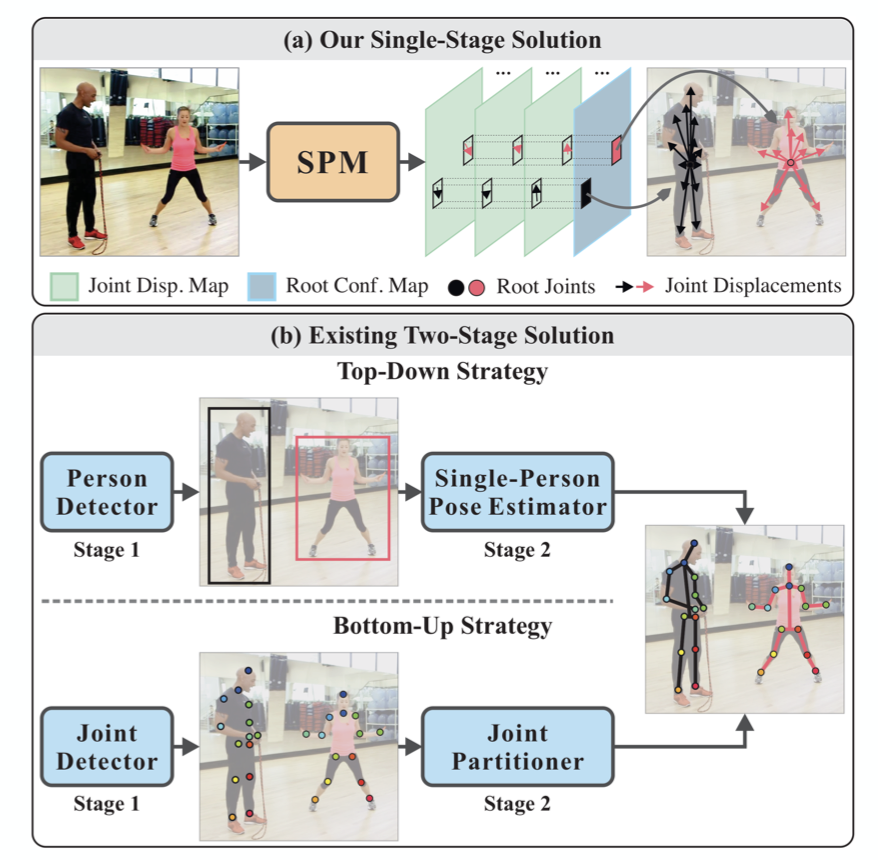
\includegraphics[width=8cm,height=5cm]{imgs/1.png}
\caption{Comparison between (a) our single-stage solution and (b) existing two-stage solution to multi-person pose estimation. The proposed SPM model directly predicts structured poses of multiple persons in a single stage, offering a more compact pipeline and attractive efficiency advantages over two-stage based top-down or bottom-up strategies. See more details in the main text.}
\end{figure}
\end{frame}

\begin{frame}
    \frametitle{Introduction}
    
    Multi-person pose estimation from a single monocular RGB image aims to simultaneously isolate and locate body joints of multiple person instances. It is a fundamental yet challenging task with broad applications in action recognition, person Re-ID, pedestrian tracking, etc.

    \vspace{0.4cm}

    \pause
    
   Existing methods typically adopt two-stage solutions. As shown in Figure(b), they either follow the top-Existing methods typically adopt two-stage solutions. As shown in Figure 1 (b), they either follow the top-down strategy that employs off-the- shelf detectors to localize person instances at first and then locates their joints individually; or the bottom-up strategy that locates all the body joints at first and then assigns them to the corresponding person. 
    
\end{frame}

\section{Background}
\subsection{Hightlight}

\begin{frame}
    \frametitle{Block and Alert}

    \begin{block}{hdhdh theorem}
        \vspace*{-\baselineskip}\setlength\belowdisplayshortskip{0.6pt}
        $$a^2 + b^2 = c^2$$
        % \vspace*{-\baselineskip}\setlength\belowdisplayshortskip{0.1pt}
        where c represents the length of the hypotenuse and 
        a and b the lengths of the triangle's other two sides.
    \end{block}
    
    \begin{alertblock}{Remark}
        \begin{itemize}
            \item the environment above is \alert{block}
            \item the environment here is \alert{alertblock}
        \end{itemize}
    \end{alertblock}

\end{frame}

\begin{frame}
    \frametitle{Proof}

    \begin{block}{Pythagorean theorem}
        \vspace*{-\baselineskip}\setlength\belowdisplayshortskip{0.1pt}
        $$a^2 + b^2 = c^2$$
        % \vspace*{-\baselineskip}\setlength\belowdisplayshortskip{0.2pt}
    \end{block}
    
    \vspace{0.4cm}

    \begin{proof}
        \vspace*{-\baselineskip}\setlength\belowdisplayshortskip{0pt}
        \begin{align*}
            &3^2 + 4^2 = 5^2\\
            &5^2 + 12^2 = 13^2
        \end{align*}
        % \vspace*{-\baselineskip}\setlength\belowdisplayshortskip{0pt}
    \end{proof}
\end{frame}

\subsection{Other Environments}

\begin{frame}{Algorithm}
    \scriptsize
    \begin{algorithm}[H]
        \KwData{this text}
        \KwResult{how to write algorithm with \LaTeX2e }
        initialization\;
        \While{not at end of this document}{
            read current\;
            \eIf{understand}{
            go to next section\;
            current section becomes this one\;
            }{
            go back to the beginning of current section\;
            }
        }
        \caption{How to write algorithms
        (copied from \href{https://en.wikibooks.org/wiki/LaTeX/Algorithms}{here})}
        \end{algorithm}
\end{frame}

\begin{frame}[fragile]
    \frametitle{An Algorithm For Finding Primes Numbers.}
    \scriptsize
    \begin{verbatim}
        int main (void)
        {
            std::vector<bool> is_prime (100, true);
            for (int i = 2; i < 100; i++)
            if (is_prime[i])
            {
                std::cout << i << " ";
                for (int j = i; j < 100; is_prime [j] = false, j+=i);
            }
            return 0;
        }
    \end{verbatim}

    \vspace{-0.7cm}

    \begin{uncoverenv}
    Note the use of \verb|\alert|.
    \end{uncoverenv}
\end{frame}

\begin{frame}{More}
    More environments such as

    \begin{itemize}
        \item Definition
        \item lemma
        \item corollary
        \item example
    \end{itemize}
\end{frame}

\section{Structured pose representation}

\subsection{Split Screen}

\begin{frame}{Minipage}
    \begin{minipage}{0.5\linewidth}
        \begin{figure}[h]
            \includegraphics[width=\textwidth]{imgs/pythagorean.jpg}
        \end{figure}
    \end{minipage}%
    \hfill
    \begin{minipage}{0.4\linewidth}
        \begin{enumerate}
            \item item
            \item another
            \item more
            \begin{itemize}
                \item first
                \item second
                \item third
            \end{itemize}
        \end{enumerate}
    \end{minipage}
\end{frame}

\begin{frame}{Columns}
    \begin{columns}
        \column{0.5\textwidth}
        This is a text in first column.
        $$E=mc^2$$
        \begin{itemize}
        \item First item
        \item Second item
        \end{itemize}
        
        \column{0.5\textwidth}
        \begin{block}{first block}
            columns achieves splitting the screen
        \end{block}
        \begin{block}{second block}
            stack block in columns
        \end{block}
        
    \end{columns}
\end{frame}

\subsection{Table}

\begin{frame}{Create Tables}
    \begin{center}
        \begin{table}[!t]  
            % \caption{Three line}
            % \label{table_time}
            \begin{tabular}{ccc}  
                \toprule   
                first&second&third\\ 
                \midrule       
                1 & 2 & 3 \\ 
                4 & 5 & 6 \\ 
                7 & 8 & 9 \\
                \bottomrule  
            \end{tabular}
        \end{table}
    \end{center}
\end{frame}

\subsection{Math}

\begin{frame}{Equation1}
    A matrix in text must be set  smaller:
    $\bigl(\begin{smallmatrix}
    a&b \\ c&d
    \end{smallmatrix} \bigr)$
    to not increase leading in a portion of text.

    \[ f(n) =
    \begin{cases}
        n/2       & \quad \text{if } n \text{ is even}\\
        -(n+1)/2  & \quad \text{if } n \text{ is odd}
    \end{cases}
    \]

    $$50 apples \times 100 apples = lots of apples^2$$
\end{frame}

\begin{frame}{Equation2}
    $$\sum_{\substack{0<i<m \\ 0<j<n }} 
      P(i,j)=\int\limits_a^b\prod P(i,j)$$

    $$P\left(A=2\middle|\frac{A^2}{B}>4\right)$$

    $$( a ), [ b ], \{ c \}, | d |, \| e \|,
    \langle f \rangle, \lfloor g \rfloor,Experiments
    \lceil h \rceil, \ulcorner i \urcorner$$
    
\end{frame}

\begin{frame}{Equation3}
    $$Q(\alpha)=\alpha_i\alpha_jy_iy_j(x_i\cdot x_j)$$

    $$Q(\alpha)=\alpha^i\alpha^jy^{(i)}y^{(j)}(x^i\cdot x^j)$$
    
    $$\Gamma=\beta+\alpha+\gamma+\rho$$
\end{frame}


\section{Single-stage multi-person pose machine}
\subsection{Regression targets}
\subsection{Network architecture}
\subsection{Training and inference}

\section{Experiments}

\section{Conclusion}

\begin{frame}{End}
    The last page.
\end{frame}